% Options for packages loaded elsewhere
\PassOptionsToPackage{unicode}{hyperref}
\PassOptionsToPackage{hyphens}{url}
\PassOptionsToPackage{dvipsnames,svgnames,x11names}{xcolor}
%
\documentclass[
  letterpaper,
  DIV=11,
  numbers=noendperiod]{scrreprt}

\usepackage{amsmath,amssymb}
\usepackage{iftex}
\ifPDFTeX
  \usepackage[T1]{fontenc}
  \usepackage[utf8]{inputenc}
  \usepackage{textcomp} % provide euro and other symbols
\else % if luatex or xetex
  \usepackage{unicode-math}
  \defaultfontfeatures{Scale=MatchLowercase}
  \defaultfontfeatures[\rmfamily]{Ligatures=TeX,Scale=1}
\fi
\usepackage{lmodern}
\ifPDFTeX\else  
    % xetex/luatex font selection
\fi
% Use upquote if available, for straight quotes in verbatim environments
\IfFileExists{upquote.sty}{\usepackage{upquote}}{}
\IfFileExists{microtype.sty}{% use microtype if available
  \usepackage[]{microtype}
  \UseMicrotypeSet[protrusion]{basicmath} % disable protrusion for tt fonts
}{}
\makeatletter
\@ifundefined{KOMAClassName}{% if non-KOMA class
  \IfFileExists{parskip.sty}{%
    \usepackage{parskip}
  }{% else
    \setlength{\parindent}{0pt}
    \setlength{\parskip}{6pt plus 2pt minus 1pt}}
}{% if KOMA class
  \KOMAoptions{parskip=half}}
\makeatother
\usepackage{xcolor}
\usepackage[margin=0.5in]{geometry}
\setlength{\emergencystretch}{3em} % prevent overfull lines
\setcounter{secnumdepth}{4}
% Make \paragraph and \subparagraph free-standing
\ifx\paragraph\undefined\else
  \let\oldparagraph\paragraph
  \renewcommand{\paragraph}[1]{\oldparagraph{#1}\mbox{}}
\fi
\ifx\subparagraph\undefined\else
  \let\oldsubparagraph\subparagraph
  \renewcommand{\subparagraph}[1]{\oldsubparagraph{#1}\mbox{}}
\fi


\providecommand{\tightlist}{%
  \setlength{\itemsep}{0pt}\setlength{\parskip}{0pt}}\usepackage{longtable,booktabs,array}
\usepackage{calc} % for calculating minipage widths
% Correct order of tables after \paragraph or \subparagraph
\usepackage{etoolbox}
\makeatletter
\patchcmd\longtable{\par}{\if@noskipsec\mbox{}\fi\par}{}{}
\makeatother
% Allow footnotes in longtable head/foot
\IfFileExists{footnotehyper.sty}{\usepackage{footnotehyper}}{\usepackage{footnote}}
\makesavenoteenv{longtable}
\usepackage{graphicx}
\makeatletter
\def\maxwidth{\ifdim\Gin@nat@width>\linewidth\linewidth\else\Gin@nat@width\fi}
\def\maxheight{\ifdim\Gin@nat@height>\textheight\textheight\else\Gin@nat@height\fi}
\makeatother
% Scale images if necessary, so that they will not overflow the page
% margins by default, and it is still possible to overwrite the defaults
% using explicit options in \includegraphics[width, height, ...]{}
\setkeys{Gin}{width=\maxwidth,height=\maxheight,keepaspectratio}
% Set default figure placement to htbp
\makeatletter
\def\fps@figure{htbp}
\makeatother
\newlength{\cslhangindent}
\setlength{\cslhangindent}{1.5em}
\newlength{\csllabelwidth}
\setlength{\csllabelwidth}{3em}
\newlength{\cslentryspacingunit} % times entry-spacing
\setlength{\cslentryspacingunit}{\parskip}
\newenvironment{CSLReferences}[2] % #1 hanging-ident, #2 entry spacing
 {% don't indent paragraphs
  \setlength{\parindent}{0pt}
  % turn on hanging indent if param 1 is 1
  \ifodd #1
  \let\oldpar\par
  \def\par{\hangindent=\cslhangindent\oldpar}
  \fi
  % set entry spacing
  \setlength{\parskip}{#2\cslentryspacingunit}
 }%
 {}
\usepackage{calc}
\newcommand{\CSLBlock}[1]{#1\hfill\break}
\newcommand{\CSLLeftMargin}[1]{\parbox[t]{\csllabelwidth}{#1}}
\newcommand{\CSLRightInline}[1]{\parbox[t]{\linewidth - \csllabelwidth}{#1}\break}
\newcommand{\CSLIndent}[1]{\hspace{\cslhangindent}#1}

\usepackage{booktabs}
\usepackage{longtable}
\usepackage{array}
\usepackage{multirow}
\usepackage{wrapfig}
\usepackage{float}
\usepackage{colortbl}
\usepackage{pdflscape}
\usepackage{tabu}
\usepackage{threeparttable}
\usepackage{threeparttablex}
\usepackage[normalem]{ulem}
\usepackage{makecell}
\usepackage{xcolor}
\usepackage{caption}
\KOMAoption{captions}{tableheading}
\usepackage{float}
\floatplacement{table}{H}
\floatplacement{image}{H}
\makeatletter
\@ifpackageloaded{tcolorbox}{}{\usepackage[skins,breakable]{tcolorbox}}
\@ifpackageloaded{fontawesome5}{}{\usepackage{fontawesome5}}
\definecolor{quarto-callout-color}{HTML}{909090}
\definecolor{quarto-callout-note-color}{HTML}{0758E5}
\definecolor{quarto-callout-important-color}{HTML}{CC1914}
\definecolor{quarto-callout-warning-color}{HTML}{EB9113}
\definecolor{quarto-callout-tip-color}{HTML}{00A047}
\definecolor{quarto-callout-caution-color}{HTML}{FC5300}
\definecolor{quarto-callout-color-frame}{HTML}{acacac}
\definecolor{quarto-callout-note-color-frame}{HTML}{4582ec}
\definecolor{quarto-callout-important-color-frame}{HTML}{d9534f}
\definecolor{quarto-callout-warning-color-frame}{HTML}{f0ad4e}
\definecolor{quarto-callout-tip-color-frame}{HTML}{02b875}
\definecolor{quarto-callout-caution-color-frame}{HTML}{fd7e14}
\makeatother
\makeatletter
\makeatother
\makeatletter
\@ifpackageloaded{bookmark}{}{\usepackage{bookmark}}
\makeatother
\makeatletter
\@ifpackageloaded{caption}{}{\usepackage{caption}}
\AtBeginDocument{%
\ifdefined\contentsname
  \renewcommand*\contentsname{Table of contents}
\else
  \newcommand\contentsname{Table of contents}
\fi
\ifdefined\listfigurename
  \renewcommand*\listfigurename{List of Figures}
\else
  \newcommand\listfigurename{List of Figures}
\fi
\ifdefined\listtablename
  \renewcommand*\listtablename{List of Tables}
\else
  \newcommand\listtablename{List of Tables}
\fi
\ifdefined\figurename
  \renewcommand*\figurename{Figure}
\else
  \newcommand\figurename{Figure}
\fi
\ifdefined\tablename
  \renewcommand*\tablename{Table}
\else
  \newcommand\tablename{Table}
\fi
}
\@ifpackageloaded{float}{}{\usepackage{float}}
\floatstyle{ruled}
\@ifundefined{c@chapter}{\newfloat{codelisting}{h}{lop}}{\newfloat{codelisting}{h}{lop}[chapter]}
\floatname{codelisting}{Listing}
\newcommand*\listoflistings{\listof{codelisting}{List of Listings}}
\makeatother
\makeatletter
\@ifpackageloaded{caption}{}{\usepackage{caption}}
\@ifpackageloaded{subcaption}{}{\usepackage{subcaption}}
\makeatother
\makeatletter
\@ifpackageloaded{tcolorbox}{}{\usepackage[skins,breakable]{tcolorbox}}
\makeatother
\makeatletter
\@ifundefined{shadecolor}{\definecolor{shadecolor}{rgb}{.97, .97, .97}}
\makeatother
\makeatletter
\makeatother
\makeatletter
\makeatother
\ifLuaTeX
  \usepackage{selnolig}  % disable illegal ligatures
\fi
\IfFileExists{bookmark.sty}{\usepackage{bookmark}}{\usepackage{hyperref}}
\IfFileExists{xurl.sty}{\usepackage{xurl}}{} % add URL line breaks if available
\urlstyle{same} % disable monospaced font for URLs
\hypersetup{
  pdftitle={Bias in Facial Classification ML Models},
  pdfauthor={Patrick Connelly; Grace Cooper; Bhavana Jonnalagadda; Carl Klein; Piya (Leo) Ngamkam; Dhairya Veera},
  colorlinks=true,
  linkcolor={blue},
  filecolor={Maroon},
  citecolor={Blue},
  urlcolor={Blue},
  pdfcreator={LaTeX via pandoc}}

\title{Bias in Facial Classification ML Models}
\author{Patrick Connelly \and Grace Cooper \and Bhavana
Jonnalagadda \and Carl Klein \and Piya (Leo) Ngamkam \and Dhairya Veera}
\date{}

\begin{document}
\maketitle
\ifdefined\Shaded\renewenvironment{Shaded}{\begin{tcolorbox}[breakable, interior hidden, borderline west={3pt}{0pt}{shadecolor}, sharp corners, boxrule=0pt, enhanced, frame hidden]}{\end{tcolorbox}}\fi

\renewcommand*\contentsname{Table of contents}
{
\hypersetup{linkcolor=}
\setcounter{tocdepth}{2}
\tableofcontents
}
\bookmarksetup{startatroot}

\hypertarget{abstract}{%
\chapter*{Abstract}\label{abstract}}
\addcontentsline{toc}{chapter}{Abstract}

\markboth{Abstract}{Abstract}

Lorem ipsum dolor sit amet, consectetur adipiscing elit, sed do eiusmod
tempor incididunt ut labore et dolore magna aliqua. Ut enim ad minim
veniam, quis nostrud exercitation ullamco laboris nisi ut aliquip ex ea
commodo consequat. Duis aute irure dolor in reprehenderit in voluptate
velit esse cillum dolore eu fugiat nulla pariatur. Excepteur sint
occaecat cupidatat non proident, sunt in culpa qui officia deserunt
mollit anim id est laborum.

\begin{center}\rule{0.5\linewidth}{0.5pt}\end{center}

\begin{tcolorbox}[enhanced jigsaw, bottomrule=.15mm, left=2mm, bottomtitle=1mm, leftrule=.75mm, coltitle=black, toprule=.15mm, breakable, opacitybacktitle=0.6, titlerule=0mm, colback=white, colbacktitle=quarto-callout-tip-color!10!white, toptitle=1mm, arc=.35mm, rightrule=.15mm, colframe=quarto-callout-tip-color-frame, opacityback=0, title=\textcolor{quarto-callout-tip-color}{\faLightbulb}\hspace{0.5em}{Report PDF and Code Location}]

A link to download the
\href{https://cuboulder-ds.github.io/5301-5000-Final-Report/STAT_5000_Final_Report.pdf}{PDF
version} of this report, and a link to the
\href{https://github.com/CUBoulder-DS/5301-5000-Final-Report}{Github
source code} for this report, are both available as icons in the top
right corner of this website.

\end{tcolorbox}

Features of Quarto:

\hypertarget{how-we-should-write-this-report}{%
\section*{How we should write this
report}\label{how-we-should-write-this-report}}
\addcontentsline{toc}{section}{How we should write this report}

\markright{How we should write this report}

\begin{itemize}
\tightlist
\item
  See Karkkainen and Joo (\protect\hyperlink{ref-fairface}{2021}) , that
  is an example on how to cite a bibliography.
\item
  Sections/title headings are automatically numbered.
\item
  Any changes you make, make sure to make a comment of your initials at
  the top of your work (INCLUDING written text) like so:
\end{itemize}

\begin{verbatim}
<!-- BJ !-->
Blah blah etc ....

OR
#BJ
r_var <- ...
\end{verbatim}

\begin{itemize}
\tightlist
\item
  Make sure to add a unique name to all code cells, and to also enable
  the following (the quarto way) (In order for a figure to be
  cross-referenceable, its label must start with the fig- prefix):
\end{itemize}

\begin{figure}

{\centering 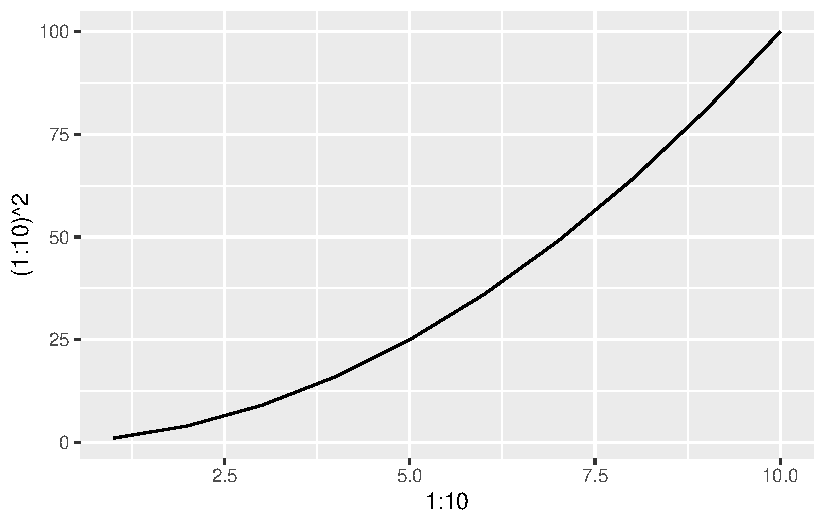
\includegraphics{index_files/figure-pdf/fig-sec1-unique-name-1.pdf}

}

\caption{\label{fig-sec1-unique-name}A caption for generated figure}

\end{figure}

\begin{itemize}
\item
  You can then refer to figures like this \texttt{@fig-sec1-unique-name}
  Figure~\ref{fig-sec1-unique-name}
\item
  Format tables doing the following
  \href{https://quarto.org/docs/reference/cells/cells-knitr.html\#tables}{Link
  here}
\item
  Do all your r work initially in your own custom \texttt{.rmd} file in
  this directory, so that it can be copy-pasted over later into the
  appropriate section (written descriptions/words can go straight into
  the \texttt{.qmd} files though). For example, Bhav's work is in
  \texttt{5000-final/BJ\_work.rmd}.
\end{itemize}

\begin{tcolorbox}[enhanced jigsaw, bottomrule=.15mm, left=2mm, bottomtitle=1mm, leftrule=.75mm, coltitle=black, toprule=.15mm, breakable, opacitybacktitle=0.6, titlerule=0mm, colback=white, colbacktitle=quarto-callout-note-color!10!white, toptitle=1mm, arc=.35mm, rightrule=.15mm, colframe=quarto-callout-note-color-frame, opacityback=0, title=\textcolor{quarto-callout-note-color}{\faInfo}\hspace{0.5em}{From the report requirements}]

A 3-5 summary of the paper. It should address the research question, the
methods, and the conclusions of your analysis.

\emph{``A good recipe for an abstract is: first sentence: specify the
general area of the paper and encourage the reader; second sentence:
specify the dataset and methods at a general level; third sentence:
specify the headline result; and a fourth sentence about
implications.''}

\end{tcolorbox}

\bookmarksetup{startatroot}

\hypertarget{introduction}{%
\chapter{Introduction}\label{introduction}}

\begin{tcolorbox}[enhanced jigsaw, bottomrule=.15mm, left=2mm, bottomtitle=1mm, leftrule=.75mm, coltitle=black, toprule=.15mm, breakable, opacitybacktitle=0.6, titlerule=0mm, colback=white, colbacktitle=quarto-callout-note-color!10!white, toptitle=1mm, arc=.35mm, rightrule=.15mm, colframe=quarto-callout-note-color-frame, opacityback=0, title=\textcolor{quarto-callout-note-color}{\faInfo}\hspace{0.5em}{From the report requirements}]

This section introduces your problem to a \textbf{non-expert} audience,
describes the context and history of the problem.

For example, if your overall project topic is on Diabetes Prevention and
Prediction, then you would use the Introduction to introduce what
diabetes is, who it affects, why prevention is important, history on
diabetes prevention, etc.

Some questions that you could answer in the introduction:

\begin{itemize}
\item
  What is the ``research question''? why is it interesting or worth
  answering?
\item
  What is the relevant background information for readers to understand
  your project? Assume that your audience\\
  is not an expert in the application field.
\item
  Is there any prior research on your topic that might be helpful for
  the audience?
\end{itemize}

The goal of the introduction it to capture the audience's interest in
your paper. An introduction that starts with ``Diabetes kills over 87
thousand people each year and in many cases may be preventable'' is more
engaging than ``This paper is about diabetes prevention''.

The introduction should be 2-4 paragraphs long.

\end{tcolorbox}

\bookmarksetup{startatroot}

\hypertarget{data}{%
\chapter{Data}\label{data}}

We describe the data here. Note that the default global setting for
Quarto is set to NOT output the code into the rendered document, aka
only including the results of any R code.

\textbf{We should include a print of the head of the dataframe of our
data, along with some sample images!!}

\hypertarget{exploration-of-source-data}{%
\section{Exploration of Source Data}\label{exploration-of-source-data}}

\begin{figure}

\begin{minipage}[t]{0.33\linewidth}

{\centering 

\raisebox{-\height}{

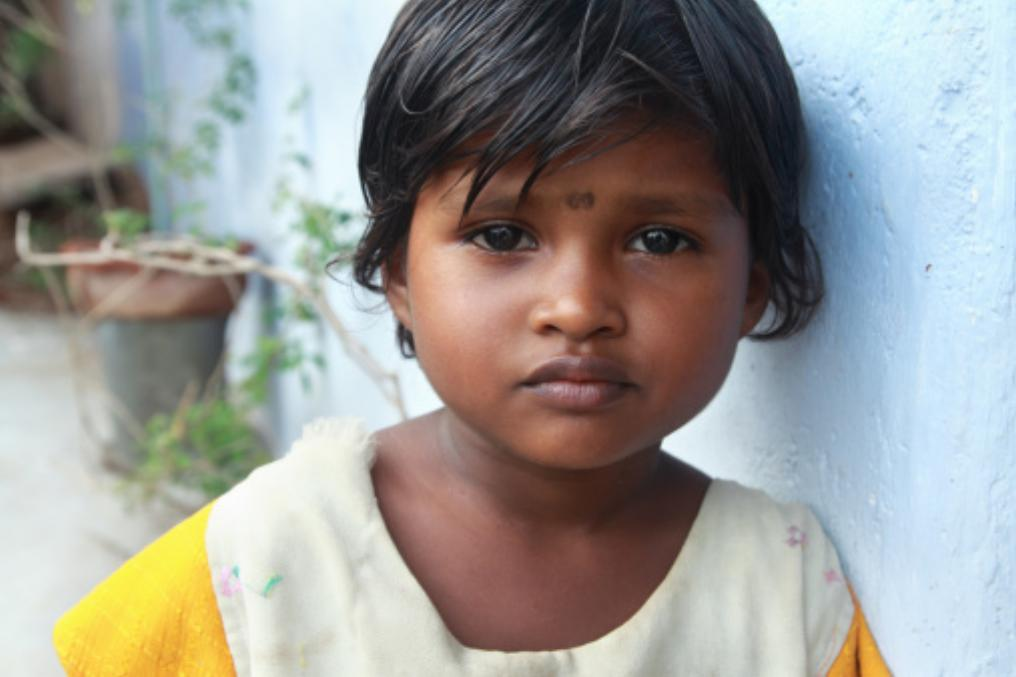
\includegraphics{images/utk_imgs/6_1_3_20161220223052131.jpg}

}

}

\subcaption{\label{fig-img1}Age=6, Gender=F, Race=Indian}
\end{minipage}%
%
\begin{minipage}[t]{0.33\linewidth}

{\centering 

\raisebox{-\height}{

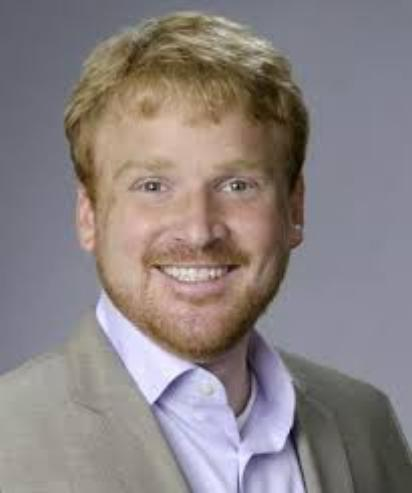
\includegraphics{images/utk_imgs/38_0_0_20170105172756958.jpg}

}

}

\subcaption{\label{fig-img2}Age=38, Gender=M, Race=White}
\end{minipage}%
%
\begin{minipage}[t]{0.33\linewidth}

{\centering 

\raisebox{-\height}{

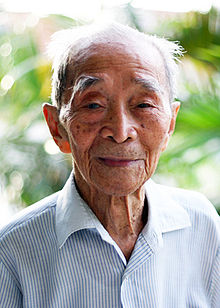
\includegraphics{images/utk_imgs/80_0_2_20170111201008732.jpg}

}

}

\subcaption{\label{fig-img3}Age=80, Gender=M, Race=Asian}
\end{minipage}%

\caption{\label{fig-faces}Example face images from the UTK dataset
(\protect\hyperlink{ref-utkDataset}{{``{UTKFace}''} 2021}) with their
associated given labels.}

\end{figure}

\begin{figure}

\begin{minipage}[t]{0.50\linewidth}

{\centering 

\raisebox{-\height}{

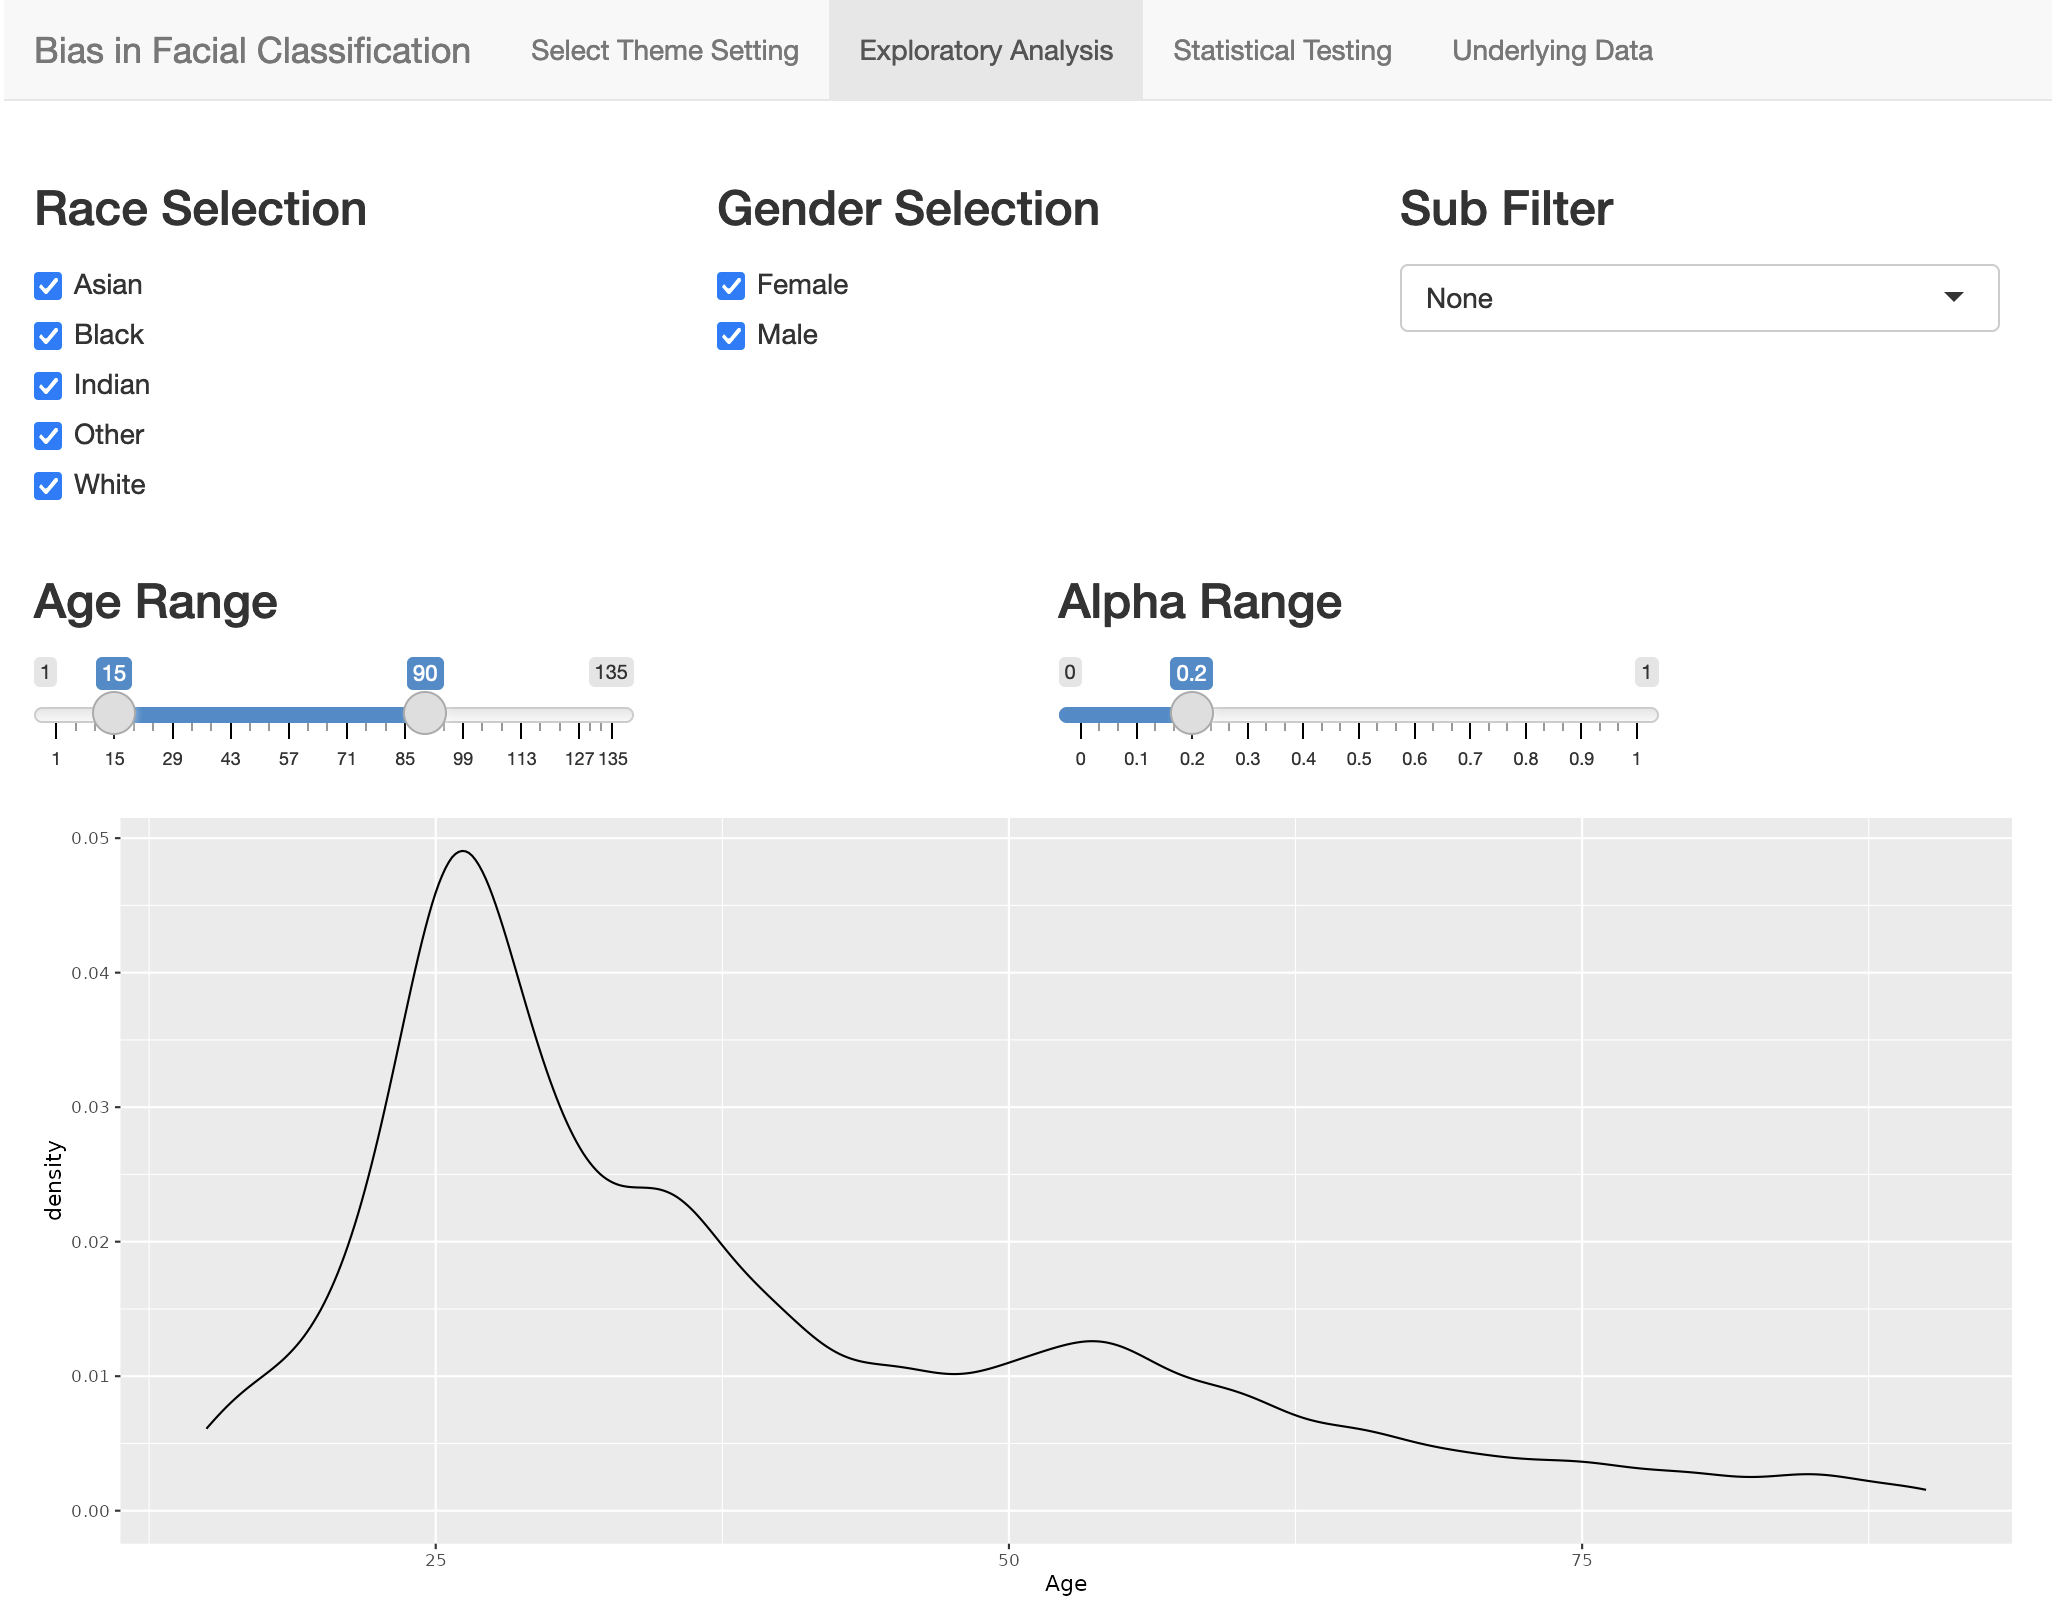
\includegraphics{"images/shiny1.png"}

}

\caption{Image data EDA}

}

\end{minipage}%
%
\begin{minipage}[t]{0.50\linewidth}

{\centering 

\raisebox{-\height}{

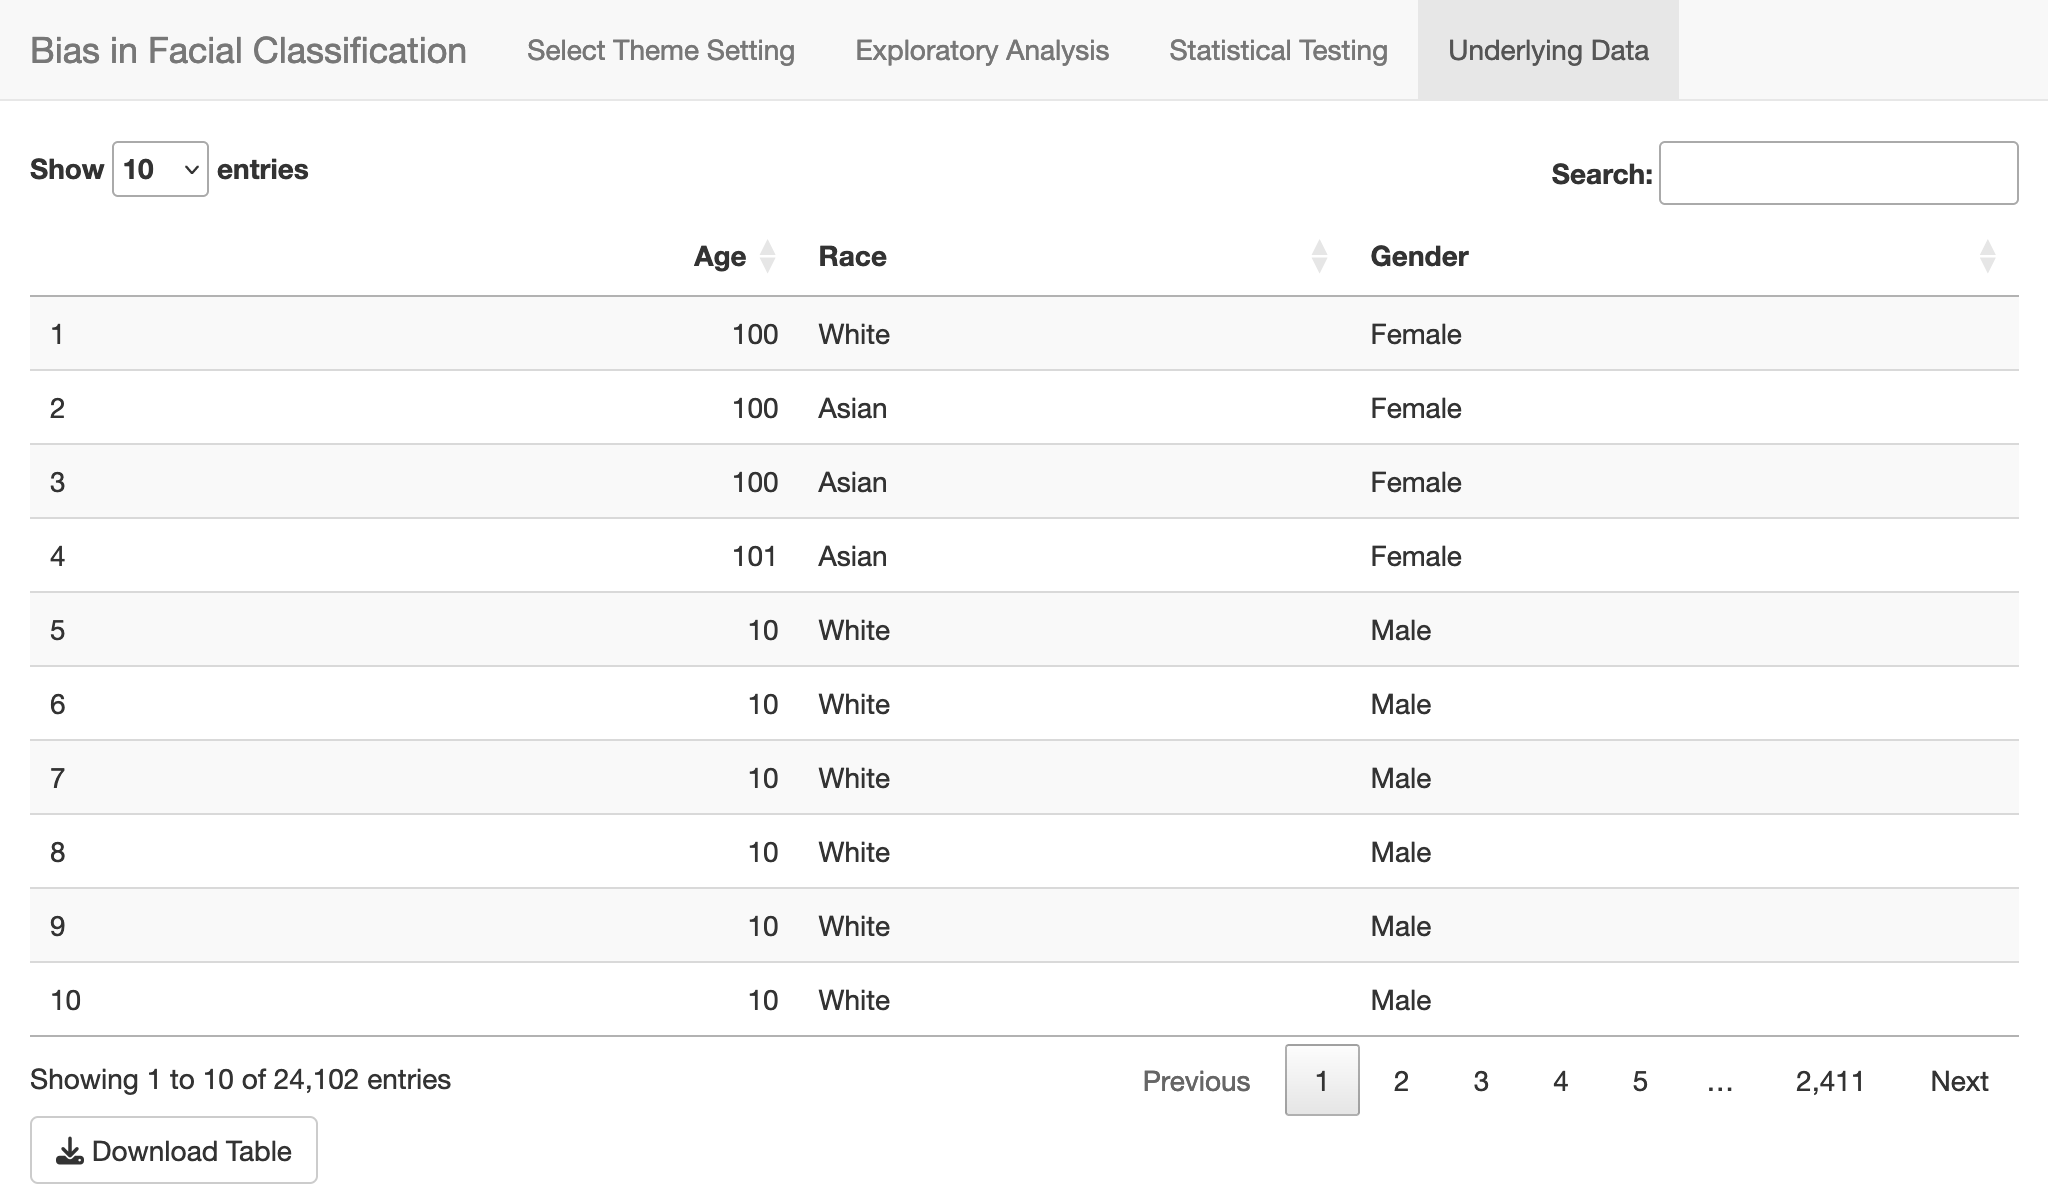
\includegraphics{"images/shiny2.png"}

}

\caption{Image dataset visualization}

}

\end{minipage}%

\caption{\label{fig-data-eda-pdf}Screenshots of the interactive figure
showcasing the distributions of various data factors in the image
dataset, and showcasing the underlying data. To see and interact with
this figure, go to
\href{https://cuboulder-ds.github.io/5301-5000-Final-Report/data.html}{the
website link}}

\end{figure}

\begin{tcolorbox}[enhanced jigsaw, bottomrule=.15mm, left=2mm, bottomtitle=1mm, leftrule=.75mm, coltitle=black, toprule=.15mm, breakable, opacitybacktitle=0.6, titlerule=0mm, colback=white, colbacktitle=quarto-callout-note-color!10!white, toptitle=1mm, arc=.35mm, rightrule=.15mm, colframe=quarto-callout-note-color-frame, opacityback=0, title=\textcolor{quarto-callout-note-color}{\faInfo}\hspace{0.5em}{From the report requirements}]

This section should describe the data you'll be using. Answer \textbf{at
least} \textbf{all} of the following questions:

\begin{itemize}
\item
  How was the data collected?
\item
  What are the sources and influences of bias in the data?
\item
  What are the important features (=columns) that you are using in your
  analysis? What do they mean?
\end{itemize}

Feel free to add anything else that you think is necessary for
understanding the paper and the context of the problem.

\end{tcolorbox}

\hypertarget{more-information-on-data}{%
\section{More information on data}\label{more-information-on-data}}

\begin{verbatim}
-- Attaching core tidyverse packages ------------------------ tidyverse 2.0.0 --
v dplyr     1.1.1     v readr     2.1.4
v forcats   1.0.0     v stringr   1.5.0
v ggplot2   3.4.2     v tibble    3.2.1
v lubridate 1.9.2     v tidyr     1.3.0
v purrr     1.0.1     
-- Conflicts ------------------------------------------ tidyverse_conflicts() --
x dplyr::filter() masks stats::filter()
x dplyr::lag()    masks stats::lag()
i Use the conflicted package (<http://conflicted.r-lib.org/>) to force all conflicts to become errors
\end{verbatim}

\begin{longtable}[]{@{}
  >{\raggedright\arraybackslash}p{(\columnwidth - 4\tabcolsep) * \real{0.1786}}
  >{\raggedright\arraybackslash}p{(\columnwidth - 4\tabcolsep) * \real{0.6349}}
  >{\raggedright\arraybackslash}p{(\columnwidth - 4\tabcolsep) * \real{0.1865}}@{}}
\toprule\noalign{}
\begin{minipage}[b]{\linewidth}\raggedright
filenames
\end{minipage} & \begin{minipage}[b]{\linewidth}\raggedright
purpose
\end{minipage} & \begin{minipage}[b]{\linewidth}\raggedright
recommendations
\end{minipage} \\
\midrule\noalign{}
\endhead
\bottomrule\noalign{}
\endlastfoot
Croped\_ff\_np.csv & Permutation evaluation (older version) for
fairface, no preprocessing on cropped images. Updated this file to look
at the same files as the uncropped dataset. & Remove from github data
folder. \\
MasterDataFrame.csv & Final master data file containing all input and
output files & Keep as-is with no changes \\
crop\_df\_np.csv & Permutation evaluation for DeepFace, cropped images,
no pre-processing & Retain; rename to PERM\_DF\_c\_np.csv \\
crop\_df\_p\_mtcnn.csv & Permutation evaluation for DeepFace, cropped
images, preprocessed with MTCNN backend. & Retain; rename to
PERM\_DF\_c\_p\_mtcnn.csv \\
crop\_df\_p\_opencv.csv & Permutation evaluation for DeepFace, cropped
images, preprocessed with OpenCV backend. & Retain; rename to
PERM\_DF\_c\_p\_opencv.csv \\
cropped\_UTK.csv & Permutation evaluation (older version), list of
cropped files to perform evaluation. & Remove from github data folder \\
cropped\_UTK\_dataset.csv & Permutation evaluation (newest version),
list of cropped files to perform evaluation. & Retain with no changes \\
cropped\_ff\_p.csv & Permutation evaluation (older version), used older
version of cropped images dataset. & Remove from github data folder. \\
joined\_permutations.csv & Permutation evaluation (newest version),
joined all permutation outputs from DeepFace and FairFace to a single
file & Retain with no changes \\
new\_ff\_c\_np.csv & Permutation evaluation (newest version), FairFaice
outputs for cropped images with no preprocessing & Retain; rename to
PERM\_FF\_c\_np.csv \\
new\_ff\_c\_p.csv & Permutation evaluation (newest version), FairFaice
outputs for cropped images with dlib preprocessing & Retain; rename to
PERM\_FF\_c\_p.csv \\
new\_ff\_uc\_np.csv & Permutation evaluation (newest version), FairFaice
outputs for uncropped images with no preprocessing & Retain; rename to
PERM\_FF\_uc\_np.csv \\
new\_ff\_uc\_p.csv & Permutation evaluation (newest version), FairFaice
outputs for uncropped images with dlib preprocessing. & Retain; rename
to PERM\_FF\_uc\_p.csv \\
non\_normalized\_DeepFace\_uncropped\_DF\_all.csv & Final dataset of
DeepFace Outputs (non-normalized) & Retain; rename to
Master\_DF\_non\_normalized.csv \\
non\_normalized\_FairFace\_uncropped\_FF\_all.csv & Final dataset of
FairFace Outputs (non-normalized) & Retain; rename to
Master\_FF\_non\_normalized.csv \\
uncropped\_DF\_all.csv & Final normalized output for DeepFace - used to
build MasterDataFrame.csv & Retain with no changes \\
uncropped\_FF\_all.csv & Final normalized output for FairFace - used to
build MasterDataFrame.csv & Retain with no changes \\
uncropped\_UTK.csv & Permutation evaluation (older version) - source
data file for iteration script & Remove from github data folder. \\
uncropped\_UTK\_dataset.csv & Permutation evaluation (newest version) -
source data file for uncropped images in iteration script & Retain with
no changes \\
uncropped\_df\_np.csv & Permutation evaluation (newest version) -
DeepFace uncropped images with no preprocessing & Retain; rename to
PERM\_DF\_uc\_np.csv \\
uncropped\_df\_p\_mtcnn.csv & Permutation Evaluation (newest version) -
DeepFace uncropped images with mtcnn preprocessing & Retain; rename to
PERM\_DF\_uc\_p\_mtcnn.csv \\
uncropped\_df\_p\_opencv.csv & Permutation Evaluation (newest version) -
DeepFace uncropped images with opencv preprocessing & Retain; rename to
PERM\_DF\_uc\_p\_opencv.csv \\
uncropped\_ff\_np.csv & Permutation Evaluation (older version) -
FairFace uncropped images with no preprocessing & Remove from github
data folder. \\
uncropped\_ff\_p.csv & Permutation Evaluation (older version) - FairFace
uncropped images with dlib preprocessing. & Remove from github data
folder. \\
\end{longtable}

\hypertarget{data-selection-utk-dataset---ln-dv}{%
\section{Data Selection (UTK Dataset) - LN
DV}\label{data-selection-utk-dataset---ln-dv}}

Motivation - has there been progress against bias?

Reference Articles from Ethics Class - Joy B's work, etc. Lots of
disparity back in 2018, how much of that still exists with free models?

\hypertarget{selected-models-ln-dv}{%
\section{Selected Models (LN DV)}\label{selected-models-ln-dv}}

Lorem ipsum

\hypertarget{fairface}{%
\subsection{FairFace}\label{fairface}}

Motivation as to how / why we came across this

\hypertarget{deepface}{%
\subsection{DeepFace}\label{deepface}}

Motivation as to how / why we came across this

\hypertarget{permutation-analysis-information}{%
\subsection{Permutation Analysis
Information}\label{permutation-analysis-information}}

\bookmarksetup{startatroot}

\hypertarget{methods}{%
\chapter{Methods}\label{methods}}

Karkkainen and Joo (\protect\hyperlink{ref-fairface}{2021})

\hypertarget{the-big-picture}{%
\section{The Big Picture}\label{the-big-picture}}

\begin{itemize}
\tightlist
\item
  Is bias prevalent in facial recognition machine learning models?
\item
  Can one model be shown to have statistically significant less bias
  than the other?
\item
  Does one model outperform the other in a statistically significant
  manner, in all aspects?
\item
  Does one model outperform the other in a statistically significant
  manner, in certain aspects?

  \begin{itemize}
  \tightlist
  \item
    This is where we can dive into ``conventional'' bias
  \end{itemize}
\end{itemize}

\begin{tcolorbox}[enhanced jigsaw, bottomrule=.15mm, left=2mm, bottomtitle=1mm, leftrule=.75mm, coltitle=black, toprule=.15mm, breakable, opacitybacktitle=0.6, titlerule=0mm, colback=white, colbacktitle=quarto-callout-note-color!10!white, toptitle=1mm, arc=.35mm, rightrule=.15mm, colframe=quarto-callout-note-color-frame, opacityback=0, title=\textcolor{quarto-callout-note-color}{\faInfo}\hspace{0.5em}{Thoughts on Bias}]

We need to be careful how we define and use bias. Statistical bias is
essentially error, and we could be crossing our definitions between
statistical bias and conventional bias.

\end{tcolorbox}

\hypertarget{measuring-performance}{%
\section{Measuring Performance}\label{measuring-performance}}

\begin{tcolorbox}[enhanced jigsaw, bottomrule=.15mm, left=2mm, bottomtitle=1mm, leftrule=.75mm, coltitle=black, toprule=.15mm, breakable, opacitybacktitle=0.6, titlerule=0mm, colback=white, colbacktitle=quarto-callout-note-color!10!white, toptitle=1mm, arc=.35mm, rightrule=.15mm, colframe=quarto-callout-note-color-frame, opacityback=0, title=\textcolor{quarto-callout-note-color}{\faInfo}\hspace{0.5em}{Note}]

This performance section is important in choosing the correct models to
ensure data integrity, however for the actual statistical tests, we'll
focused on more common statistics like mean and proportion.

\end{tcolorbox}

There are four main measures of performance when evaluating a model:

\begin{itemize}
\tightlist
\item
  \textbf{Accuracy}
\item
  \textbf{Precision}
\item
  \textbf{Recall}
\item
  \textbf{F1-Score}
\end{itemize}

Each of these performance measures has their own place in evaluating
models, however, to begin to explain the differences between these
models we should start with concepts of positive and negative outcomes.

\begin{itemize}
\tightlist
\item
  \textbf{True Positive:} predicted positive, was actually positive
  (correct)
\item
  \textbf{False Positive:} predicted positive, was actually negative
  (incorrect)
\item
  \textbf{True Negative:} predicted negative, was actually negative
  (correct)
\item
  \textbf{False Negative:} predicted negative, was actually positive
  (incorrect)
\end{itemize}

These outcomes can be visualized on a confusion matrix. In the image
below, green are correct predictions while red are incorrect
predictions.

\begin{figure}

{\centering 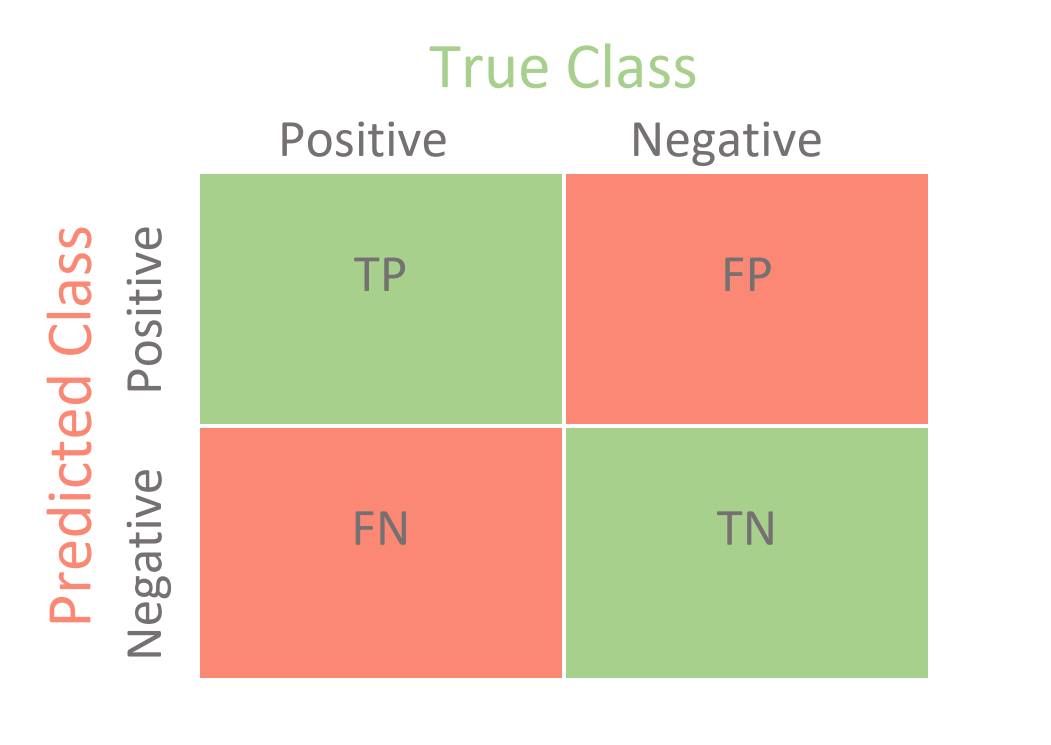
\includegraphics{images/confusion_matrix.png}

}

\caption{confusion\_matrix}

\end{figure}

\hypertarget{accuracy}{%
\subsection{Accuracy}\label{accuracy}}

\textbf{Accuracy} is the ratio of correct predictions to all
predictions. In other words, the total of the green squares divided by
the entire matrix. This is arguably the most common concept of measuring
performance.

\(Acccuracy = \frac{TP+TN}{TP + TN + FN}\)

\hypertarget{precision}{%
\subsection{Precision}\label{precision}}

\textbf{Precision} is the ratio of true positives to the total number of
positives (true positive + true negative).

\(Precision = \frac{TP}{TP+FP}\)

\hypertarget{recall}{%
\subsection{Recall}\label{recall}}

\textbf{Recall} is the ratio of true positives to the number of total
correct predictions (true positive + false negative).

\(Recall = \frac{TP}{TP+FN}\)

\hypertarget{f1-score}{%
\subsection{F1-Score}\label{f1-score}}

\textbf{F1-Score}* is known as the harmonic mean between precision and
recall. \textbf{Precision} and \textbf{Recall} are useful in their own
rights, but the f1-Score is useful in the fact it's a balanced
combination of both precision and recall.

F1-Score \(= \frac{2 * Precision * Recall}{Precision + Recall}\)

\hypertarget{hypothesis-testing}{%
\section{Hypothesis Testing}\label{hypothesis-testing}}

Our data consists of three main sets, the source input data, the
Fairface output data, and the Deepface output data.

We'll be creating our hypothesis tests by treating the source data as
the basis for the original assumptions (our \emph{null hypotheses}), and
then using the output from Fairface and Deepface to test for
statistically significant differences. Gaining a statistically
significant result would allow us to reject our \emph{null hypothesis}
in favor of the \emph{alternative hypothesis}. In other words, rejecting
the original assumption means there is a statistically large enough
difference between the source data and output data, and could indicate a
bias in model.

We'll be testing across different subsets contained within the data, as
listed below:

\hypertarget{demographics}{%
\subsection{Demographics}\label{demographics}}

\begin{itemize}
\tightlist
\item
  Age Group
\item
  Gender
\item
  Race
\end{itemize}

\hypertarget{demographics-subgroups}{%
\subsection{Demographics' Subgroups}\label{demographics-subgroups}}

\begin{itemize}
\tightlist
\item
  Age Group (9 groups)

  \begin{itemize}
  \tightlist
  \item
    0-2
  \item
    3-9
  \item
    10-19
  \item
    20-29
  \item
    30-39
  \item
    40-49
  \item
    50-59
  \item
    60-69
  \item
    70-130
  \end{itemize}
\item
  Gender (2 groups)

  \begin{itemize}
  \tightlist
  \item
    Female
  \item
    Male
  \end{itemize}
\item
  Race (5 groups)

  \begin{itemize}
  \tightlist
  \item
    Asian
  \item
    Black
  \item
    Indian
  \item
    Other
  \item
    White
  \end{itemize}
\end{itemize}

\hypertarget{the-general-proportion-tests}{%
\subsection{The General Proportion
Tests}\label{the-general-proportion-tests}}

Our hypothesis tests will be testing different proportions within these
subgroups between the source data and the output data.

The general format of our hypothesis tests will be:

\(H_0: p = p_{\text{Source Data Subset}}\)

\(H_A: p \neq p_{\text{Source Data Subset}}\)

With the following test statistic:

\(\frac{\sqrt{n}(\hat{p} - p)}{\sqrt{p(1 - p)}}\)

With the p-value being calculated by:

\(P(|Z| > \hat{p} | H_0)\)

\(= P(|Z| > \frac{\sqrt{n}(\hat{p} - p)}{\sqrt{p(1 - p)}})\),

where

\begin{itemize}
\tightlist
\item
  \(n\): output data subset size
\item
  \(\hat{p}\): output data subset proportion
\item
  \(p\): source data subset proportion
\end{itemize}

\hypertarget{notation}{%
\subsection{Notation}\label{notation}}

Before we list the specific tests, we should introduce some notation.

Let \(R\) be race, then
\(R \in \{Asian, Black, Indian, Other, White\} = \{A, B, I, O, W\}\)

Let \(G\) be gender, then \(G \in \{Female, Male\} = \{F, M\}\)

Let \(A\) be age, then
\(A \in \{[0,2], [3,9], [10,19], [20,29], [30,39], [40,49], [50,59], [60,69], [70,130]\} = \{1, 2, 3, 4, 5, 6, 7, 8, 9\}\)

Let \(D\) be the dataset, then
\(D \in \{Source, Fairface, Deepface\} = \{D_0, D_f, D_d\}\)

\hypertarget{more-specific-proportion-tests}{%
\subsection{More Specific Proportion
Tests}\label{more-specific-proportion-tests}}

Using this notation, we can simplify our nomenclature for testing a
certain proportion of an overall demographic.

For example, we can test if the proportion of \emph{Female} in the
Fairface output is statistically different than the proportion of
\emph{Female} from the source.

Hypothesis Test:

\(H_0: p_F = p_{F|D_0}\)

\(H_A: p_F \neq p_{F|D_0}\)

P-value Calculation:

\(P(|Z| > \frac{\sqrt{n}(\hat{p} - p)}{\sqrt{p(1 - p)}})\),

where

\begin{itemize}
\tightlist
\item
  \(p = p_{F|D_0}\): proportion of females from the source data
\item
  \(\hat{p} = p_{F|D_f}\): proportion of females from the fairface
  output
\item
  \(n = n_{F \cup M|D_f}\): number of data points in the gender subset
  form the fairface output
\end{itemize}

Additionally, we could test for different combinations of subsets within
demographics. For instance, if we wanted to test for a statistically
significant difference between the proportion of those who
\emph{Female}, given that they were \emph{Black}, then we could write a
hypothesis test like:

\(H_0: p_{F|B} = p_{F|D_0 \cap B}\)

\(H_A: p_{F|B} \neq p_{F|D_0 \cap B}\)

P-value Calculation:

\(P(|Z| > \frac{\sqrt{n}(\hat{p} - p)}{\sqrt{p(1 - p)}})\),

where

\begin{itemize}
\tightlist
\item
  \(p = p_{F|D_0 \cap B}\): proportion of females from the source data,
  given they were black
\item
  \(\hat{p} = p_{F|D_f \cap B}\): proportion of females from the
  fairface output, given they were black
\item
  \(n = n_{F \cup M|D_f \cap B}\): number of data points in the gender
  subset form the fairface output, given they were black.
\end{itemize}

These were two specific hypothesis tests, however, we'll be testing many
combinations of these parameters and reporting back on any significant
findings.

\begin{tcolorbox}[enhanced jigsaw, bottomrule=.15mm, left=2mm, bottomtitle=1mm, leftrule=.75mm, coltitle=black, toprule=.15mm, breakable, opacitybacktitle=0.6, titlerule=0mm, colback=white, colbacktitle=quarto-callout-note-color!10!white, toptitle=1mm, arc=.35mm, rightrule=.15mm, colframe=quarto-callout-note-color-frame, opacityback=0, title=\textcolor{quarto-callout-note-color}{\faInfo}\hspace{0.5em}{From the report requirements}]

Also can be called ``Analyses''

This section might contain several subsections as needed.

\begin{itemize}
\item
  At least one subsection should describe the exploratory data analysis
  you did.
\item
  What modifications were necessary to make the dataset ready for
  analysis? (e.g.~dealing with missing values, removing certain rows,
  replacing/cleaning text values, binning, etc)
\item
  Describe the analyses you did to answer the question of interest.
  \textbf{Explain why you believe these methods are appropriate.}
\item
  At least one subsection should describe the exploratory data analysis
  you did.
\item
  What modifications were necessary to make the dataset ready for
  analysis? (e.g.~dealing with missing values, removing certain rows,
  replacing/cleaning text values, binning, etc)
\item
  Describe the analyses you did to answer the question of interest.
  \textbf{Explain why you believe these methods are appropriate.}
\item
  At least one subsection should describe the exploratory data analysis
  you did.
\item
  What modifications were necessary to make the dataset ready for
  analysis? (e.g.~dealing with missing values, removing certain rows,
  replacing/cleaning text values, binning, etc)
\item
  Describe the analyses you did to answer the question of interest.
  \textbf{Explain why you believe these methods are appropriate.}
\end{itemize}

Some methods we learn in this class include distribution comparison,
correlation analysis, and hypothesis testing. You are required to
include hypothesis tests into the project, but feel free to use
additional methods to tell a good story about the data.

\end{tcolorbox}

\hypertarget{standardizing-output}{%
\section{Standardizing output}\label{standardizing-output}}

The model outputs for both FairFace and DeepFace do not conform to the
categories provided within the University of Tennessee - Knoxville (UTK)
dataset. We elected to take the outputs from each model and modify them
based upon the categories specified in the UTK dataset, namely:

\begin{itemize}
\item
  ``{[}race{]} is an integer from 0 to 4, denoting White, Black, Asian,
  Indian, and Others (like Hispanic, Latino, Middle Eastern).''
\item
  ``{[}gender{]} is either 0 (male) or 1 (female)''
\item
  ``{[}age{]} is an integer from 0 to 116, indicating the age''
\end{itemize}

\hypertarget{from-fairface}{%
\subsection{From FairFace}\label{from-fairface}}

\begin{itemize}
\item
  \textbf{Race}: The FairFace classification model had two options - one
  for ``fair7'' and one for ``fair4.'' The latter provided predictions
  of race in the following categories: {[}White, Black, Asian,
  Indian{]}. Of key note, the model omitted ``Other'' categories as
  listed in the race category for the UTK dataset. However, the
  ``fair7'' model provides predictions across {[}White, Black,
  Latino\_Hispanic, East Asian, Southeast Asian, Indian, Middle
  Eastern{]}. We elected to use the the fair7 model, and to refactor the
  output categories to match those of the UTK dataset. Namely, we
  refactored instances of Middle Eastern and Latino\_Hispanic as
  ``Other,'' and instances of ``East Asian'' and ``Southeast Asian'' as
  ``Asian''
\item
  \textbf{Age}: FairFace only provides a predicted age range as opposed
  to a specific, single, predicted age as a string. To enable comparison
  of actual values to the predicted values, we maintained this column as
  a categorical variable, and split it into a lower and upper bound of
  predicted age as an integer. This split will allow us to determine
  whether or not the prediction correctly binned the age
  (i.e.~\(lowerBound \leq actualAge \leq upperBound\)), and if not - how
  far outside of those bounds the actual age lay.
\item
  \textbf{Gender}: no change to outputs of ``Male'' and ``Female.''
\end{itemize}

\hypertarget{from-deepface}{%
\subsection{From DeepFace}\label{from-deepface}}

\begin{itemize}
\item
  \textbf{Race}: Racial categorical output from DeepFace includes the
  following categories {[}``middle eastern'', ``asian'', ``white'',
  ``latino hispanic'', ``black'', ``indian''{]}
\item
  \textbf{Age}: DeepFace provides a prediction of a single, specific,
  predicted age. We elected to match the predicted age to be the same
  range as would be predicted by Fair Face. For example, if DeepFace
  predicts an age like ``19,'' we assign it the same matching category
  as it would have in FairFace - ``10-19.'' From there, we also split
  this category into an upper and lower bound. In spite of the fact that
  DeepFace does not provide any bounds or ranges on its age prediction
  outputs, to have a similar and fair comparison of both models, we give
  it those same upper and lower bounds for equitable comparison.
\item
  \textbf{Gender}: DeepFace outputs are ``Man'' and ``Woman'', and we
  refactor those values to ``Male'' and ``Female'' respectively.
\end{itemize}

\hypertarget{evaluating-permutations-of-inputs-and-models-for-equitable-evaluation}{%
\section{Evaluating Permutations of Inputs and Models for Equitable
Evaluation}\label{evaluating-permutations-of-inputs-and-models-for-equitable-evaluation}}

Aside from the differences in the outputs of each model in terms of age,
race, and gender, there are also substantial differences between
FairFace and DeepFace in terms of their available settings when
attempting to categorize an image in each of these categories.

The need for this permutation evaluation rose from some initial
scripting and testing of these models on a small sample of images from
another facial dataset - the Asian Face Age Dataset (need citation
here). We immediately grew concerned with DeepFace's performance using
default settings (namely, enforcing requirement to detect a face prior
to categorization, and using OpenCV as the default detection backend).
Running these initial scripting tests, we encountered a failure rate in
DeepFace of approximately 70\% in identifying and categorizing an image
of a face.

We performed further exploratory analysis on both models in light of
these facts, and sought some specific permutations of settings to
determine what settings may provide the most fair and equitable
comparison of the models prior to proceeding to further analysis.

\hypertarget{deepface-analysis-options}{%
\subsection{DeepFace Analysis Options}\label{deepface-analysis-options}}

DeepFace has a robust degree of avaialble settings when performing
facial categorization and recognition. These include enforcing facial
detection prior to classification of an image, as well as 8 different
facial detection models to detect a face prior to categorization. The
default of these settings is OpenCV detection with detection enabled.
Other detection backends include ssd, dlib, mtcnn, retinaface,
mediapipe, yolov8, yunet, and fastmtcnn.

In a Python 3.8 environment, attempting to run detections using dlib,
retinaface, mediapipe, yolov8, and yunet failed to run, or failed to
install the appropriate models directly from source during exeuction.
Repairing any challenges or issues with the core functionality of
DeepFace and FairFace's code is outside the scope of our work, and as
such, we have excluded any of these non-functioning models from our
permutation evaluation.

\hypertarget{fairface-analysis-options}{%
\subsection{FairFace Analysis Options}\label{fairface-analysis-options}}

The default script from FairFace provided no options via its command
line script to change settings. It uses dlib/resnet34 models for facial
detection and image pre-processing, and uses its own fair4 and fair7
models for categorization. There are no other options or flags that can
be set by a user when processing a batch of images.

We converted the simple script to a class in Python without addressing
any feature bugs or errors in the underlying code. This change provided
us some additional options when performing the analysis of an input
image using FairFace - namely, the ability to analyze and categorize an
image with or without facial detection, similar to the functionality of
DeepFace. FairFace remains limited in the fact that is only detection
model backend is built in dlib, but this change gives us more options
when considering what type of images to use and what settings to use on
both models before generating our final dataset for analysis.

\hypertarget{specific-permutations}{%
\subsection{Specific Permutations}\label{specific-permutations}}

With the above options in mind, we designed the following permutations
for evaluation on a subset of the UTK dataset:

\begin{longtable}[]{@{}llll@{}}
\toprule\noalign{}
Detection & Detection Model & Image Source & Results Output \\
\midrule\noalign{}
\endhead
\bottomrule\noalign{}
\endlastfoot
Enabled & FairFace=Dlib; DeepFace=OpenCV & Pre-cropped &
new\_ff\_c\_p.csv, crop\_df\_p\_opencv.csv \\
Enabled & FairFace=Dlib; DeepFace=OpenCV & In-The-Wild &
new\_ff\_uc\_p.csv, uncropped\_df\_p\_opencv.csv \\
Enabled & FairFace=Dlib; DeepFace=mtcnn & Pre-cropped &
new\_ff\_c\_p.csv, crop\_df\_p\_mtcnn.csv \\
Enabled & FairFace=Dlib; DeepFace=mtcnn & In-The-Wild &
new\_ff\_uc\_p.csv, uncropped\_df\_p\_mtcnn.csv \\
Disabled & FairFace,DeepFace=None & Pre-cropped & new\_ff\_c\_np.csv,
cropped\_df\_np.csv \\
Disabled & FairFace,DeepFace=None & In-The-Wild & new\_ff\_uc\_np.csv,
uncropped\_df\_np.csv \\
\end{longtable}

We processed each of the above setting permutations againnst
approximately 9800 images, consisting of images from part 1 of 3 from
the UTK datset. Each of the cropped images (cropped\_UTK\_dataset.csv)
and uncropped images (uncropped\_UTK\_dataset.csv) came from the same
underlying subject in each image; the only difference between each image
was whether or not it was pre-processed before evaluation by each model.

\hypertarget{permutation-sample-results-ln-dv}{%
\subsection{Permutation Sample Results (LN \&
DV)}\label{permutation-sample-results-ln-dv}}

(enforcement of facial detection, detection backend model, and cropped
images vs.~faces in-the-wild)

\hypertarget{setting-selection}{%
\subsection{Setting Selection}\label{setting-selection}}

Upon completion of our evaluation, we determined the settings that gave
both models the best chance of success included enabling facial
detection with mtcnn for DeepFace and Dlib for FairFace on uncropped
images.

From there, we proceeded to process the entirety of the UTK dataset
using these settings. The only exception are 4 images that did not
conform to UTK's naming convention to identify age, gender, and race of
the subject in the image.

We wrote a script, MasterScript.py, to enable us to perform batch
iteration of images and generate output files. When processing, we
generated both the non-normalized output content and normalized output
content.

Due to the resource-intensive design of FairFace, our script enables
multiprocessing of FairFace to allow for multiple simultaneous instances
of the FairFace class as a pool of worker threads to iterate over all of
the source data.

We attempted the same methodology for DeepFace, but encountered issues
with silent errors and halting program execution when iterating over all
images using DeepFace. To alleviate this challenge, we processed
DeepFace in a single-threaded manner, and with smaller portions of the
dataset vs.~pursuing an all-in-one go execution. We proceeded to store
the data for each of these smaller runs in multiple output files to
combine once we completed all processing requirements.

The following table outlines the output files.

The last file, MasterDataFrame.csv, is the final output of our
evaluation. This file is in the following format, with the following
column definitions:

\begin{longtable}[]{@{}lll@{}}
\toprule\noalign{}
Column Name & Definition & Data Type \\
\midrule\noalign{}
\endhead
\bottomrule\noalign{}
\endlastfoot
img\_path & Relative path location of the file within the UTK dataset &
character vector \\
file & The filename of each file within the UTK dataset & character
vector \\
src\_age & The age of the subject in each image from the UTK dataset &
integer \\
src\_gender & The gender of the subject in each image from the UTK
dataset & character vector \\
src\_race & The race of the subject in each image from the UTK datset &
character vector \\
src\_timestamp & The time at which the image was submitted to the UTK
dataset & character vector \\
src\_age\_grp & The age group (matching age ranges from the FairFace
outputs) for each image in the UTK dataset & character vector \\
pred\_model & The model used to produce the predicted output (FairFace
or DeepFace) & character vector \\
pred\_race & The race of the subject in the image predicted by the given
prediction model & character vector \\
pred\_gender & The gender of the subject in the image predicted by the
given prediction model & character vector \\
pred\_age\_DF\_only & The integer-predicted age by DeepFace of the
subject in the image & integer \\
pred\_age\_grp & The age group of the subject in the image predicted by
the given prediction model & character vector \\
pred\_age\_lower & The integer lower bound of the predicted age group &
integer \\
pred\_age\_upper & The integer upper bound of the predicted age group &
integer \\
\end{longtable}

\bookmarksetup{startatroot}

\hypertarget{results}{%
\chapter{Results}\label{results}}

\section{Tabbed example output}

\begin{figure}

\begin{minipage}[t]{0.50\linewidth}

{\centering 

\raisebox{-\height}{

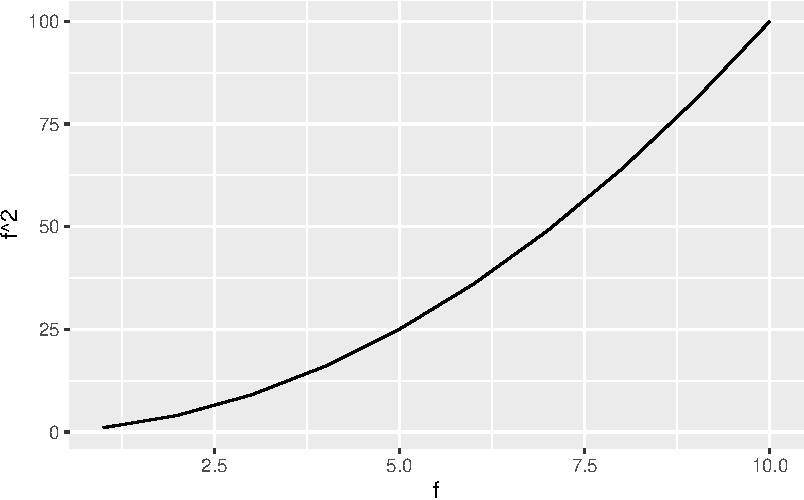
\includegraphics{results_files/figure-pdf/fig-sec4-ex2-1.pdf}

}

}

\subcaption{\label{fig-sec4-ex2-1}Subcap}
\end{minipage}%
%
\begin{minipage}[t]{0.50\linewidth}

{\centering 

\raisebox{-\height}{

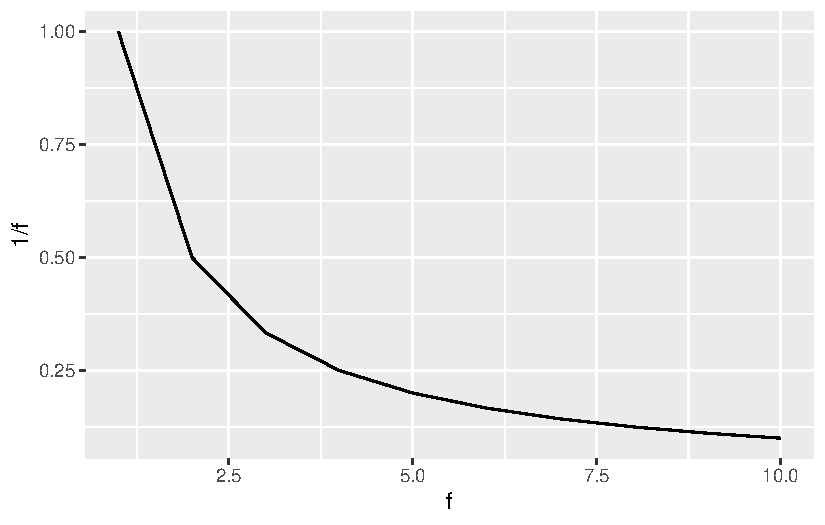
\includegraphics{results_files/figure-pdf/fig-sec4-ex2-2.pdf}

}

}

\subcaption{\label{fig-sec4-ex2-2}Subcap 2}
\end{minipage}%

\caption{\label{fig-sec4-ex2}ANother example caption}

\end{figure}

\section{Example outout}

\begin{verbatim}
 [1]  1  2  3  4  5  6  7  8  9 10
\end{verbatim}

\begin{tcolorbox}[enhanced jigsaw, bottomrule=.15mm, left=2mm, bottomtitle=1mm, leftrule=.75mm, coltitle=black, toprule=.15mm, breakable, opacitybacktitle=0.6, titlerule=0mm, colback=white, colbacktitle=quarto-callout-note-color!10!white, toptitle=1mm, arc=.35mm, rightrule=.15mm, colframe=quarto-callout-note-color-frame, opacityback=0, title=\textcolor{quarto-callout-note-color}{\faInfo}\hspace{0.5em}{From the report requirements}]

Describe the results of your analysis using visualizations, descriptive
statistics, tables and similar.

Don't focus too much on the implications in this section -- that's what
the next section is for. Just present the numbers/graphs.

\end{tcolorbox}

\hypertarget{model-output}{%
\section{Model Output}\label{model-output}}

The two models, DeepFace and FairFace, were run on the dataset described
previously. In Figure~\ref{fig-output-hists}, one can see the results of
the predictions done by each model, by each factor that was considered:
age, gender, and race. Note that the histogram distributions match the
correct (source dataset) distributions, so we can see exactly the
difference between what was provided and what was predicted, along with
how well each model did on each category within each factor.

\begin{figure}

\begin{minipage}[t]{0.50\linewidth}

{\centering 

\raisebox{-\height}{

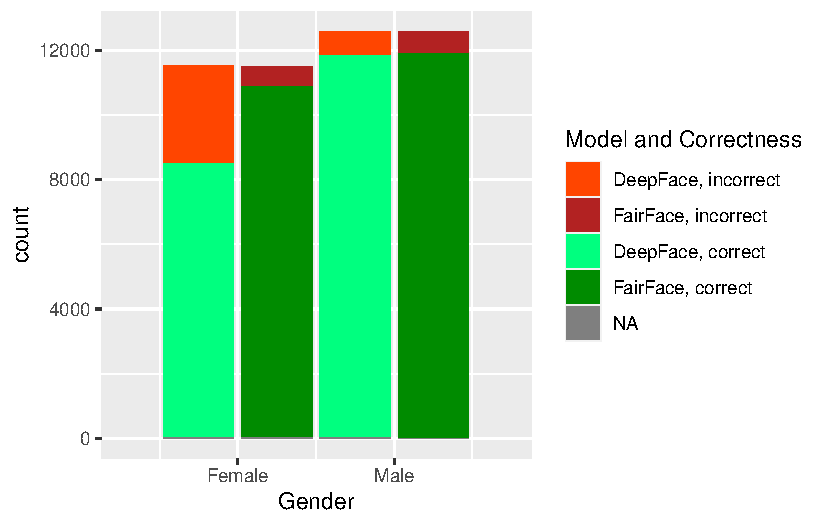
\includegraphics{results_files/figure-pdf/fig-output-hists-1.pdf}

}

}

\subcaption{\label{fig-output-hists-1}Gender predictions}
\end{minipage}%
%
\begin{minipage}[t]{0.50\linewidth}

{\centering 

\raisebox{-\height}{

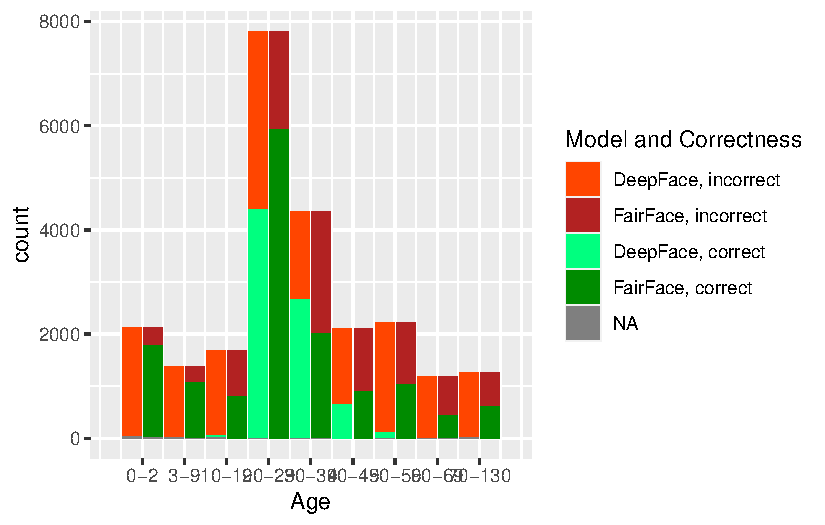
\includegraphics{results_files/figure-pdf/fig-output-hists-2.pdf}

}

}

\subcaption{\label{fig-output-hists-2}Age predictions}
\end{minipage}%
\newline
\begin{minipage}[t]{0.50\linewidth}

{\centering 

\raisebox{-\height}{

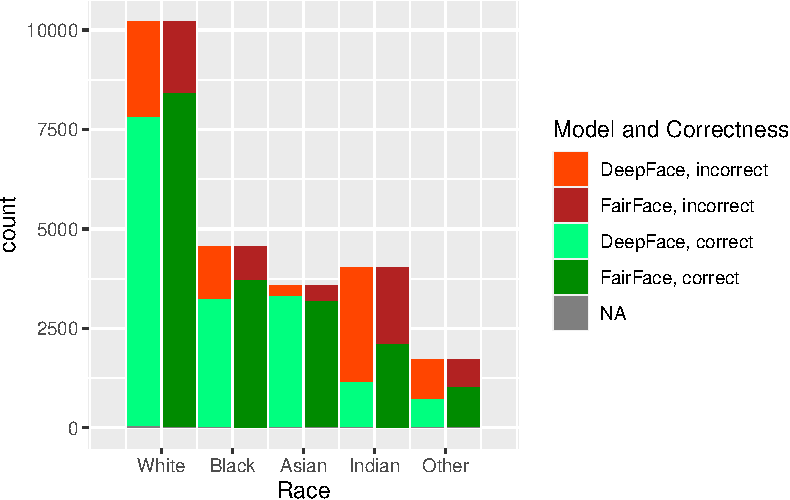
\includegraphics{results_files/figure-pdf/fig-output-hists-3.pdf}

}

}

\subcaption{\label{fig-output-hists-3}Race predictions}
\end{minipage}%

\caption{\label{fig-output-hists}Histograms of the output from DeepFace
and FairFace, with correct vs incorrect values colored. Note that the
distributions match the correct (source dataset) distributions.}

\end{figure}

\hypertarget{model-performance}{%
\section{Model Performance}\label{model-performance}}

For each category and model, we calculate the F1 score and accuracy, as
described in section 3. The results are summarized in
Table~\ref{tbl-model-perf}. Cell values are colored according to the
strength of the metric.

\hypertarget{tbl-model-perf}{}
\begin{longtable}{lrrrr}
\caption{\label{tbl-model-perf}Table of F1 score and accuracy, by each category evaluated by the models }\tabularnewline

\toprule
 & \multicolumn{2}{c}{\textbf{FairFace}} & \multicolumn{2}{c}{\textbf{DeepFace}} \\ 
\cmidrule(lr){2-3} \cmidrule(lr){4-5}
Category & \textbf{F1} & \textbf{Accuracy} & \textbf{F1} & \textbf{Accuracy} \\ 
\midrule\addlinespace[2.5pt]
\multicolumn{5}{l}{\textbf{Age}} \\ 
\midrule\addlinespace[2.5pt]
0-2 & \cellcolor[HTML]{CAFF70}{0.8959757} & \cellcolor[HTML]{CAFF70}{0.9172888} & \cellcolor[HTML]{FFA07A}{NA} & 0.5000000 \\ 
3-9 & 0.7176035 & \cellcolor[HTML]{CAFF70}{0.8772778} & \cellcolor[HTML]{FFA07A}{NA} & 0.5000000 \\ 
10-19 & 0.5052498 & 0.7211461 & \cellcolor[HTML]{FFA07A}{0.047860101} & 0.5055825 \\ 
20-29 & 0.7332922 & \cellcolor[HTML]{CAFF70}{0.8050592} & 0.505432596 & 0.6217793 \\ 
30-39 & \cellcolor[HTML]{FFA07A}{0.4670003} & 0.6741504 & \cellcolor[HTML]{FFA07A}{0.378631811} & 0.6275447 \\ 
40-49 & \cellcolor[HTML]{FFA07A}{0.3943970} & 0.6786302 & \cellcolor[HTML]{FFA07A}{0.227627841} & 0.5866155 \\ 
50-59 & \cellcolor[HTML]{FFA07A}{0.4633983} & 0.7049843 & \cellcolor[HTML]{FFA07A}{0.080167306} & 0.5137145 \\ 
60-69 & \cellcolor[HTML]{FFA07A}{0.3739425} & 0.6708204 & \cellcolor[HTML]{FFA07A}{0.001612903} & \cellcolor[HTML]{FFA07A}{0.4991769} \\ 
70-130 & 0.6270661 & 0.7383514 & \cellcolor[HTML]{FFA07A}{NA} & 0.5000000 \\ 
\midrule\addlinespace[2.5pt]
\multicolumn{5}{l}{\textbf{Race}} \\ 
\midrule\addlinespace[2.5pt]
White & \cellcolor[HTML]{CAFF70}{0.8610399} & \cellcolor[HTML]{CAFF70}{0.8788455} & \cellcolor[HTML]{CAFF70}{0.809546093} & \cellcolor[HTML]{CAFF70}{0.8365916} \\ 
Black & \cellcolor[HTML]{CAFF70}{0.8684858} & \cellcolor[HTML]{CAFF70}{0.8997692} & 0.796499445 & \cellcolor[HTML]{CAFF70}{0.8462797} \\ 
Asian & \cellcolor[HTML]{CAFF70}{0.8948932} & \cellcolor[HTML]{CAFF70}{0.9338128} & 0.703897491 & \cellcolor[HTML]{CAFF70}{0.9005150} \\ 
Indian & 0.6402458 & 0.7488102 & \cellcolor[HTML]{FFA07A}{0.409248134} & 0.6310597 \\ 
Other & \cellcolor[HTML]{FFA07A}{0.3087473} & 0.7105889 & \cellcolor[HTML]{FFA07A}{0.238902067} & 0.6283106 \\ 
\midrule\addlinespace[2.5pt]
\multicolumn{5}{l}{\textbf{Gender}} \\ 
\midrule\addlinespace[2.5pt]
 & \cellcolor[HTML]{CAFF70}{0.9429153} & \cellcolor[HTML]{CAFF70}{0.9453080} & \cellcolor[HTML]{CAFF70}{0.819770248} & \cellcolor[HTML]{CAFF70}{0.8402892} \\ 
\bottomrule
\end{longtable}

\hypertarget{hypothesis-testing-1}{%
\section{Hypothesis Testing}\label{hypothesis-testing-1}}

\begin{tabu} to \linewidth {>{\raggedright}X>{\raggedleft}X>{\raggedleft}X>{\raggedleft}X>{\raggedleft}X>{\raggedleft}X}
\hline
Test cateogry & Null Proportion & FairFace Proportion & FairFace P-Value & DeepFace Proportion & DeepFace P-Value\\
\hline
\textbf{0-2} & 0.0880010 & 0.0762941 & 0.0000000 & 0.0000000 & 0\\
\hline
\textbf{3-9} & 0.0568832 & 0.0664564 & 0.0000000 & 0.0000000 & 0\\
\hline
\textbf{10-19} & 0.0697867 & 0.0606451 & 0.0000000 & 0.0206211 & 0\\
\hline
\textbf{20-29} & 0.3238735 & 0.3480138 & 0.0000000 & 0.3987029 & 0\\
\hline
\textbf{30-39} & 0.1802755 & 0.1762899 & 0.1075659 & 0.4047312 & 0\\
\hline
\textbf{40-49} & 0.0872542 & 0.1023619 & 0.0000000 & 0.1467177 & 0\\
\hline
\textbf{50-59} & 0.0923160 & 0.0930638 & 0.6884418 & 0.0268158 & 0\\
\hline
\textbf{60-69} & 0.0490831 & 0.0490640 & 0.9890528 & 0.0024113 & 0\\
\hline
\textbf{70-130} & 0.0525268 & 0.0278112 & 0.0000000 & 0.0000000 & 0\\
\hline
\end{tabu}

\begin{tabu} to \linewidth {>{\raggedright}X>{\raggedleft}X>{\raggedleft}X>{\raggedleft}X>{\raggedleft}X>{\raggedleft}X}
\hline
Test cateogry & Null Proportion & FairFace Proportion & FairFace P-Value & DeepFace Proportion & DeepFace P-Value\\
\hline
\textbf{White} & 0.4240727 & 0.3854136 & 0.0000000 & 0.3757120 & 0\\
\hline
\textbf{Black} & 0.1891129 & 0.1652484 & 0.0000000 & 0.1479233 & 0\\
\hline
\textbf{Asian} & 0.1487843 & 0.1448259 & 0.0842652 & 0.2408847 & 0\\
\hline
\textbf{Indian} & 0.1670816 & 0.1030675 & 0.0000000 & 0.0611150 & 0\\
\hline
\textbf{Other} & 0.0709485 & 0.2014445 & 0.0000000 & 0.1743649 & 0\\
\hline
\end{tabu}

\begin{tabu} to \linewidth {>{\raggedright}X>{\raggedleft}X>{\raggedleft}X>{\raggedleft}X>{\raggedleft}X>{\raggedleft}X}
\hline
Test cateogry & Null Proportion & FairFace Proportion & FairFace P-Value & DeepFace Proportion & DeepFace P-Value\\
\hline
\textbf{Female} & 0.4780101 & 0.4797642 & 0.5857219 & 0.3833202 & 0\\
\hline
\textbf{Male} & 0.5219899 & 0.5202358 & 0.5857219 & 0.6166798 & 0\\
\hline
\end{tabu}

\begin{tabu} to \linewidth {>{\raggedright}X>{\raggedright}X>{\raggedleft}X>{\raggedleft}X>{\raggedleft}X>{\raggedleft}X>{\raggedleft}X}
\hline
Test Category & Test Condition & Null Proportion & FairFace Proportion & FairFace P-Value & DeepFace Proportion & DeepFace P-Value\\
\hline
\textbf{Female} & White & 0.4572938 & 0.4888530 & 0.0000000 & 0.4355428 & 3.32e-05\\
\hline
\textbf{Female} & Asian & 0.5415505 & 0.5431356 & 0.8509504 & 0.3879876 & 0.00e+00\\
\hline
\textbf{Female} & Black & 0.4872751 & 0.4649586 & 0.0048467 & 0.2405846 & 0.00e+00\\
\hline
\textbf{Female} & Indian & 0.4325801 & 0.4430125 & 0.2940541 & 0.3496599 & 0.00e+00\\
\hline
\textbf{Female} & Other & 0.5508772 & 0.4477643 & 0.0000000 & 0.3972341 & 0.00e+00\\
\hline
\textbf{Male} & White & 0.5427062 & 0.5111470 & 0.0000000 & 0.5644572 & 3.32e-05\\
\hline
\textbf{Male} & Asian & 0.4584495 & 0.4568644 & 0.8509504 & 0.6120124 & 0.00e+00\\
\hline
\textbf{Male} & Black & 0.5127249 & 0.5350414 & 0.0048467 & 0.7594154 & 0.00e+00\\
\hline
\textbf{Male} & Indian & 0.5674199 & 0.5569875 & 0.2940541 & 0.6503401 & 0.00e+00\\
\hline
\textbf{Male} & Other & 0.4491228 & 0.5522357 & 0.0000000 & 0.6027659 & 0.00e+00\\
\hline
\end{tabu}

\hypertarget{updated-table-version-with-data-from-carl-bav}{%
\subsection{Updated Table Version with Data from Carl,
Bav}\label{updated-table-version-with-data-from-carl-bav}}

\begin{tabular}{l|l|r|r|r|r|r|r}
\hline
Race & Category & F1\_f & Accuracy\_f & F1\_d & Accuracy\_d & f\_p\_value & d\_p\_value\\
\hline
White & 0-2 & 0.9039010 & 0.9334307 & NA & 0.5000000 & 0.0000000 & 0.0000000\\
\hline
White & 3-9 & 0.7503392 & 0.8668432 & NA & 0.5000000 & 0.0526039 & 0.0000000\\
\hline
White & 10-19 & 0.5638298 & 0.7330315 & 0.0634648 & 0.5102546 & 0.0000000 & 0.0000000\\
\hline
White & 20-29 & 0.6697460 & 0.8072440 & 0.4256326 & 0.6363584 & 0.0000000 & 0.0000000\\
\hline
White & 30-39 & 0.4731553 & 0.6821608 & 0.3884765 & 0.6486930 & 0.0410025 & 0.0000000\\
\hline
White & 40-49 & 0.3847156 & 0.6683039 & 0.2224248 & 0.5730236 & 0.0000001 & 0.0000000\\
\hline
White & 50-59 & 0.4832502 & 0.7046059 & 0.0890599 & 0.5086819 & 0.0252436 & 0.0000000\\
\hline
White & 60-69 & 0.3545817 & 0.6482054 & NaN & 0.4978778 & 0.0064930 & 0.0000000\\
\hline
White & 70-130 & 0.6342183 & 0.7403000 & NA & 0.5000000 & 0.0000000 & 0.0000000\\
\hline
White & Male & 0.9595281 & 0.9566327 & 0.8892356 & 0.8697687 & 0.0000000 & 0.0000332\\
\hline
White & Female & 0.9526238 & 0.9566327 & 0.8556585 & 0.8697687 & 0.0000000 & 0.0000332\\
\hline
Asian & 0-2 & 0.9164589 & 0.9301909 & NA & 0.5000000 & 0.0000018 & 0.0000000\\
\hline
Asian & 3-9 & 0.7140255 & 0.9111790 & NA & 0.5000000 & 0.0000000 & 0.0000000\\
\hline
Asian & 10-19 & 0.3798450 & 0.6944844 & 0.0395257 & 0.5023622 & 0.2105900 & 0.0000000\\
\hline
Asian & 20-29 & 0.8557951 & 0.8792496 & 0.5572885 & 0.5947638 & 0.0001071 & 0.0000000\\
\hline
Asian & 30-39 & 0.5069357 & 0.7042053 & 0.2992611 & 0.6258649 & 0.0000180 & 0.0000000\\
\hline
Asian & 40-49 & 0.3320463 & 0.6626378 & 0.1520190 & 0.5924407 & 0.3360992 & 0.0000000\\
\hline
Asian & 50-59 & 0.4608696 & 0.7272357 & 0.0898876 & 0.5273304 & 0.9201820 & 0.0066069\\
\hline
Asian & 60-69 & 0.4141414 & 0.7581786 & NaN & 0.4988555 & 0.0000225 & 0.0000000\\
\hline
Asian & 70-130 & 0.7441860 & 0.8051278 & NA & 0.5000000 & 0.0000000 & 0.0000000\\
\hline
Asian & Male & 0.8914286 & 0.8993780 & 0.7940330 & 0.7911354 & 0.8509504 & 0.0000000\\
\hline
Asian & Female & 0.9058670 & 0.8993780 & 0.7630232 & 0.7911354 & 0.8509504 & 0.0000000\\
\hline
Black & 0-2 & 0.8854962 & 0.9026663 & NA & 0.5000000 & 0.2466380 & 0.0000000\\
\hline
Black & 3-9 & 0.7400881 & 0.8957332 & NA & 0.5000000 & 0.0039351 & 0.0000000\\
\hline
Black & 10-19 & 0.3784787 & 0.6953003 & 0.0164609 & 0.5032694 & 0.0003683 & 0.0000000\\
\hline
Black & 20-29 & 0.6875152 & 0.7184594 & 0.5880567 & 0.6367203 & 0.0000002 & 0.0272015\\
\hline
Black & 30-39 & 0.4518681 & 0.6299581 & 0.4413203 & 0.5975793 & 0.0001798 & 0.0000000\\
\hline
Black & 40-49 & 0.3260274 & 0.6301481 & 0.1827542 & 0.5549318 & 0.3688694 & 0.0000300\\
\hline
Black & 50-59 & 0.3565062 & 0.6523810 & 0.0549451 & 0.5097384 & 0.0421863 & 0.0000000\\
\hline
Black & 60-69 & 0.3508772 & 0.6526201 & 0.0104712 & 0.5019317 & 0.0012999 & 0.0000000\\
\hline
Black & 70-130 & 0.4086022 & 0.6383490 & NA & 0.5000000 & 0.0000000 & 0.0000000\\
\hline
Black & Male & 0.9637681 & 0.9625782 & 0.8471279 & 0.8126869 & 0.0048467 & 0.0000000\\
\hline
Black & Female & 0.9615732 & 0.9625782 & 0.7724665 & 0.8126869 & 0.0048467 & 0.0000000\\
\hline
Indian & 0-2 & 0.8132911 & 0.8442303 & NA & 0.5000000 & 0.0000000 & 0.0000000\\
\hline
Indian & 3-9 & 0.6047619 & 0.8704983 & NA & 0.5000000 & 0.0012086 & 0.0000000\\
\hline
Indian & 10-19 & 0.4719764 & 0.7130687 & NaN & 0.4916753 & 0.0164656 & 0.0000000\\
\hline
Indian & 20-29 & 0.7635997 & 0.8073113 & 0.4985183 & 0.5964419 & 0.0000012 & 0.0000262\\
\hline
Indian & 30-39 & 0.4403292 & 0.6658402 & 0.3380175 & 0.5981267 & 0.0000000 & 0.0000000\\
\hline
Indian & 40-49 & 0.4636872 & 0.7199526 & 0.2997904 & 0.6063907 & 0.0000000 & 0.7150347\\
\hline
Indian & 50-59 & 0.4649351 & 0.6957273 & 0.0581655 & 0.5119443 & 0.0073901 & 0.0000000\\
\hline
Indian & 60-69 & 0.4563758 & 0.7281110 & NaN & 0.4997424 & 0.0107443 & 0.0000000\\
\hline
Indian & 70-130 & 0.5882353 & 0.7307264 & NA & 0.5000000 & 0.0103013 & 0.0000078\\
\hline
Indian & Male & 0.9574045 & 0.9525160 & 0.8897860 & 0.8485028 & 0.2940541 & 0.0000000\\
\hline
Indian & Female & 0.9452171 & 0.9525160 & 0.8234153 & 0.8485028 & 0.2940541 & 0.0000000\\
\hline
Other & 0-2 & 0.9193246 & 0.9396536 & NA & 0.5000000 & 0.0000000 & 0.0000000\\
\hline
Other & 3-9 & 0.7043189 & 0.8634606 & NA & 0.5000000 & 0.0000091 & 0.0000000\\
\hline
Other & 10-19 & 0.5460317 & 0.7189416 & 0.0597015 & 0.4968047 & 0.0000000 & 0.0000000\\
\hline
Other & 20-29 & 0.7610619 & 0.8012345 & 0.4800507 & 0.5252573 & 0.0292985 & 0.1160161\\
\hline
Other & 30-39 & 0.5017182 & 0.7224076 & 0.3505618 & 0.6391325 & 0.0000000 & 0.0000000\\
\hline
Other & 40-49 & 0.4630542 & 0.7061024 & 0.3068783 & 0.6199385 & 0.0000000 & 0.0000000\\
\hline
Other & 50-59 & 0.5000000 & 0.7472707 & 0.0983607 & 0.5278998 & 0.0000000 & 0.0091047\\
\hline
Other & 60-69 & 0.6000000 & 0.8318627 & NA & 0.5000000 & 0.0000000 & 0.0008174\\
\hline
Other & 70-130 & 0.5000000 & 0.6666667 & NA & 0.5000000 & 0.0000000 & 0.0001216\\
\hline
Other & Male & 0.9047310 & 0.9136183 & 0.8216482 & 0.8341205 & 0.0000000 & 0.0000000\\
\hline
Other & Female & 0.9216000 & 0.9136183 & 0.8379888 & 0.8341205 & 0.0000000 & 0.0000000\\
\hline
\end{tabular}

\hypertarget{statistical-power}{%
\subsection{Statistical Power}\label{statistical-power}}

\[
\beta = P\bigg(\bigg|\frac{\sqrt{n}\cdot\hat{p}-p_a}{\sqrt{p_a(1-p_a)}}\bigg|\geq\frac{\sqrt{n}\cdot p_0-p_a}{\sqrt{p_0(1-p_0)}}\bigg)
\]

Our selected level of significance is 99.7\% (3-sigma). Type-II error is
denoted by \(\beta\) above, and Power will be \(1-\beta\)

With \(p_0\) being our \emph{assumed} population proportion (from the
source dataset and what we used in our tests), \(p_a\) being the
\emph{actual} population proportion (from one or more of the below
methods), \(n\) being the number of predicted members of a racial group
(i.e.~``Indian''),

\begin{itemize}
\item
  For Gender - assume that sex at birth is a bernoulli trial, over time,
  the proportion for both genders should be 0.5
\item
  For age groups - assume that age has a true normal distribution. Each
  race may have different means and standard deviations for their
  distribution of age, but still adhere to a normal distribution. The
  ``population'' proportions may be a bit more challenging to calculate,
  but under this framework, we may be able to get there.

  \begin{itemize}
  \item
    May be able to get via bootstrapping the source dataset, average age
    by race - I think that's what we did in our last project?
  \item
    Could look at external data? May not have time to look through
    everything.
  \end{itemize}
\end{itemize}

\[
\frac{\sqrt{n_M}\cdot(\bar{p}_M-p_S)}{\sqrt{p_S\cdot(1-P_S)}}
\]

\bookmarksetup{startatroot}

\hypertarget{conclusions}{%
\chapter{Conclusions}\label{conclusions}}

\begin{tcolorbox}[enhanced jigsaw, bottomrule=.15mm, left=2mm, bottomtitle=1mm, leftrule=.75mm, coltitle=black, toprule=.15mm, breakable, opacitybacktitle=0.6, titlerule=0mm, colback=white, colbacktitle=quarto-callout-note-color!10!white, toptitle=1mm, arc=.35mm, rightrule=.15mm, colframe=quarto-callout-note-color-frame, opacityback=0, title=\textcolor{quarto-callout-note-color}{\faInfo}\hspace{0.5em}{From the report requirements}]

\begin{itemize}
\item
  Summarize what the paper has done, and discuss the implications of
  your Results.
\item
  Explicitly connect the results to the research question.
\item
  Discuss how you would you extend this research
\end{itemize}

Like the introduction, this section should be written with a
\textbf{non-expert} in mind. A person should be able to read
Introduction+Conclusion and get a rough idea of the meaning and
significance of your paper

\end{tcolorbox}

\bookmarksetup{startatroot}

\hypertarget{references}{%
\chapter*{References}\label{references}}
\addcontentsline{toc}{chapter}{References}

\markboth{References}{References}

\hypertarget{refs}{}
\begin{CSLReferences}{1}{0}
\leavevmode\vadjust pre{\hypertarget{ref-fairface}{}}%
Karkkainen, Kimmo, and Jungseock Joo. 2021. {``FairFace: Face Attribute
Dataset for Balanced Race, Gender, and Age for Bias Measurement and
Mitigation.''} In \emph{Proceedings of the IEEE/CVF Winter Conference on
Applications of Computer Vision}, 1548--58.

\leavevmode\vadjust pre{\hypertarget{ref-utkDataset}{}}%
{``{UTKFace}.''} 2021. \emph{UTKFace}.
\url{https://susanqq.github.io/UTKFace}.

\end{CSLReferences}



\end{document}
